\newpage
\section[Day 6: Cardinality]{Cardinality}

\subsection{Cardinality}

{ \color{blue} Definition 6.1.1: Onto and 1-1 Mapping } 

	\begin{adjustbox}{minipage=14cm, right, vspace=0.1cm 0cm}
		Suppose for every x $\in$ A, there is an associated f(x) $\in$ B.

		Then f maps A into B = f: A $\rightarrow$ B.
		\begin{itemize}[leftmargin=1cm, itemsep=0.4em]
			\item If f(A) = B, then f maps A onto B.
			
			\item If for each y $\in$ B, f$^{-1}$(y) consist of at most one x $\in$ A
				where f$^{-1}$(y$_1$) = x$_1$ $\neq$ x$_2$ = f$^{-1}$(y$_2$) for y$_1$ $\neq$ y$_2$,
				then f is a 1-1 mapping of A into B.
		\end{itemize}
	\end{adjustbox}

\begin{figure}[h]
	\centering
	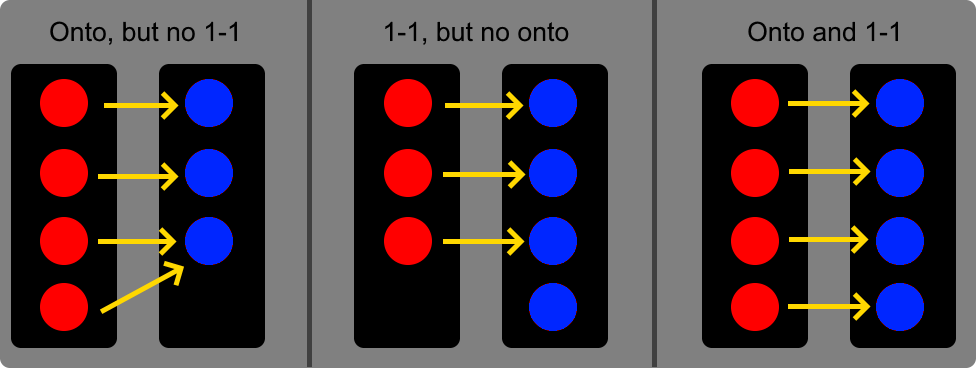
\includegraphics[scale=0.3]{Images/6.1.1.png}
\end{figure}

{ \color{blue} Definition  6.1.2: 1-1 Correspondence} 

	\begin{adjustbox}{minipage=14cm, right, vspace=0.1cm 0cm}
		Sets A and B are equivalent {\color{lblue} (have the same cardinality)} if there is
		a 1-1 onto function f: A $\rightarrow$ B. {\color{lblue} (1-1 correspondence between A and B)}
		Then:

		\qquad A $\sim$ B

		If f: A $\rightarrow$ B is 1-1 and onto, then
		there is a f$^{-1}$: B $\rightarrow$ A that is 1-1 and onto. \\
	\end{adjustbox}

{ \color{blue} Definition 6.1.3: Countability } 
	\begin{itemize}[leftmargin=1cm, itemsep=0.4em]
		\item A is {\color{lblue} finite} if A $\sim$ J$_n$ = \{0, 1, ..., n\}
			for some n $\in$ $\mathbb{N}$
		\item A is {\color{lblue} infinite} if A is not finite
		\item A is {\color{lblue} countably infinite} if A $\sim$ J = $\mathbb{Z}_+$
		\item A is {\color{lblue} uncountable} if A is not finite or countably infinite
		\item A is {\color{lblue} at most countable} if A is finite or countably infinite \\
	\end{itemize}

{ \color{purple} Example 6.1.4 } 

	\qquad $\mathbb{Z}$ is countably infinite

{ \color{magenta} \underline{Proof} } 

	Let f: $\mathbb{Z}_+$ $\rightarrow$ $\mathbb{Z}$

	\hspace{0.5cm} f(n) = 
	$
	\begin{cases}
		\frac{n}{2} & \text{n is even} \\
		-\frac{n-1}{2} & \text{n is odd} \\
	\end{cases}
	$

	So 1 $\mapsto$ 0 , 2 $\mapsto$ 1, 3 $\mapsto$ -1, 4 $\mapsto$ 2, 5 $\mapsto$ -2 , etc.
	Thus, $\mathbb{Z}$ $\sim$ $\mathbb{Z}_+$. \\ 

\newpage

{ \color{blue} Definition 6.1.5: Pigeonhole Principle } 

	\qquad If A is finite, A is not equivalent to any proper set of A.

	\begin{figure}[h]
	\centering
	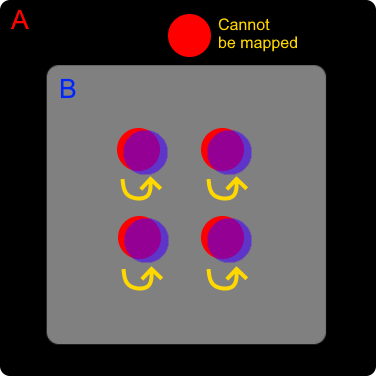
\includegraphics[scale=0.5]{Images/6.1.5.png}
\end{figure}

{ \color{red} Theorem 6.1.6: Infinite subsets of countable sets are countable } 

	\qquad An infinite subset E of a countably infinite set A is countably infinite.

{ \color{magenta} \underline{Proof} } 

	Let E $\subset$ A be an infinite subset.
	For every distinct $x_i$ $\in$ A, let x = \{ $x_1, x_2, ...$ \}.

	Let $n_1$ be smallest integer such that x$_{n_1}$ $\in$ E.

	Then let $n_2$ be the smallest integer where $n_2$ $>$ $n_1$ such that x$_{n_2}$ $\in$ E.

	Repeat the process to create sequence f(k) = \{ $x_{n_1}, x_{n_2}, ... , x_{n_k} , ...$ \}.

	Thus, there is a 1-1 correspondence between E and $\mathbb{Z}_+$ so
	E is countably infinite.

\begin{figure}[h]
	\centering
	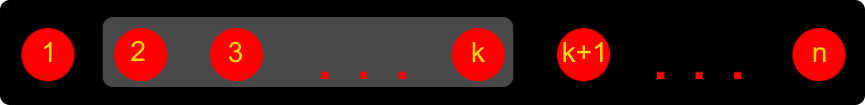
\includegraphics[scale=0.5]{Images/6.1.6.png}
\end{figure}

\subsection{ Set of Sets } 

{ \color{blue} Definition 6.2.1: Union and Intersection } 

	\begin{adjustbox}{minipage=14cm, right, vspace=0.1cm 0cm}
		Let sets $\Omega$,B be such that for each x $\in$ $\Omega$,
		there is an associated E$_x$ $\subset$ B.
		\begin{itemize}[leftmargin=1cm, itemsep=0.4em]
			\item E = $\cup_{x=1}^{n}$ E$_x$ only if for every x $\in$ E, x $\in$ E$_x$ for
				at least one x $\in$ $\Omega$.

			\item P = $\cap_{x=1}^{n}$ E$_x$ only if for every x $\in$ P, x $\in$ E$_x$ for
				all x $\in$ $\Omega$.
		\end{itemize}
		with properties:
	\end{adjustbox}

	\begin{enumerate}[label=(\alph*), leftmargin=2cm, itemsep=0.4em]
		\item A $\cup_{}^{}$ B = B $\cup_{}^{}$ A
			\hspace{4cm} A $\cap_{}^{}$ B = B $\cap_{}^{}$ A

		\item (A $\cup_{}^{}$ B) $\cup_{}^{}$ C = A $\cup_{}^{}$ (B $\cup_{}^{}$ C)
			\hspace{1.6cm} (A $\cap_{}^{}$ B) $\cap_{}^{}$ C = A $\cap_{}^{}$ (B $\cap_{}^{}$ C)

		\item A $\subset$ A $\cup_{}^{}$ B
			\hspace{4.8cm} (A $\cap_{}^{}$ B) $\subset$ A

		\item If A $\subset$ B, then A $\cup_{}^{}$ B = B and A $\cap_{}^{}$ B = A

			{ \color{magenta} \underline{Proof} } 
			
				If x $\in$ A $\cup_{}^{}$ B, then x $\in$ A or/and x $\in$ B.
				\begin{itemize}[leftmargin=1cm, itemsep=0.4em]
					\item If x $\in$ A, since A $\subset$ B, then x $\in$ B.
						Then, (A $\cup_{}^{}$ B) $\subset$ B.

					\item If x $\in$ B, then immediately (A $\cup_{}^{}$ B) $\subset$ B.
				\end{itemize}
				If x $\in$ B, then x $\in$ A $\cup_{}^{}$ B so B $\subset$ (A $\cup_{}^{}$ B).
				Thus, A $\cup_{}^{}$ B = B.

				\vspace{0.5cm}

				If x $\in$ A $\cap_{}^{}$ B, then x $\in$ A and x $\in$ B.
				Thus, (A $\cap_{}^{}$ B) $\subset$ A.

				If x $\in$ A, since A $\subset$ B, then x $\in$ B so x $\in$ A $\cap_{}^{}$ B.
				Thus, A $\subset$ (A $\cap_{}^{}$ B).

				Thus, A $\cap_{}^{}$ B = A.

		\item A $\cap_{}^{}$ (B $\cup_{}^{}$ C) = (A $\cap_{}^{}$ B) $\cup_{}^{}$ (A $\cap_{}^{}$ C)

			{ \color{magenta} \underline{Proof} } 
			
				If x $\in$ A $\cap_{}^{}$ (B $\cup_{}^{}$ C), then x $\in$ A
				and (x $\in$ B or/and x $\in$ C).
				\begin{itemize}[leftmargin=1cm, itemsep=0.4em]
					\item If x $\in$ B, then x $\in$ (A $\cap_{}^{}$ B) so
						x $\in$ (A $\cap_{}^{}$ B) $\cup_{}^{}$ (A $\cap_{}^{}$ C).

					\item If x $\in$ C, then x $\in$ (A $\cap_{}^{}$ C) so
						x $\in$ (A $\cap_{}^{}$ B) $\cup_{}^{}$ (A $\cap_{}^{}$ C).
				\end{itemize}
				Thus, A $\cap_{}^{}$ (B $\cup_{}^{}$ C)
				$\subset$ (A $\cap_{}^{}$ B) $\cup_{}^{}$ (A $\cap_{}^{}$ C).
				
				If x $\in$ (A $\cap_{}^{}$ B) $\cup_{}^{}$ (A $\cap_{}^{}$ C),
				then x $\in$ A and (x $\in$ B or/and x $\in$ C).

				Thus, (A $\cap_{}^{}$ B) $\cup_{}^{}$ (A $\cap_{}^{}$ C)
				$\subset$ A $\cap_{}^{}$ (B $\cup_{}^{}$ C).

				Thus, A $\cap_{}^{}$ (B $\cup_{}^{}$ C)
				= (A $\cap_{}^{}$ B) $\cup_{}^{}$ (A $\cap_{}^{}$ C).

		\item A $\cup_{}^{}$ (B $\cap_{}^{}$ C) = (A $\cup_{}^{}$ B) $\cap_{}^{}$ (A $\cup_{}^{}$ C)

			{ \color{magenta} \underline{Proof} } 
			
			If x $\in$ A $\cup_{}^{}$ (B $\cap_{}^{}$ C), then
			x $\in$ A or/and (x $\in$ B and x $\in$ C).
			\begin{itemize}[leftmargin=1cm, itemsep=0.4em]
				\item If x $\in$ A, then x $\in$ (A $\cup_{}^{}$ B)
					and x $\in$ (A $\cup_{}^{}$ C)
					so A $\cup_{}^{}$ (B $\cap_{}^{}$ C) $\subset$
					(A $\cup_{}^{}$ B) $\cap_{}^{}$ (A $\cup_{}^{}$ C).

				\item If x $\in$ B,C, then x $\in$ (A $\cup_{}^{}$ B)
					and x $\in$ (A $\cup_{}^{}$ C)
					so A $\cup_{}^{}$ (B $\cap_{}^{}$ C) $\subset$
					(A $\cup_{}^{}$ B) $\cap_{}^{}$ (A $\cup_{}^{}$ C).
			\end{itemize}
			If x $\in$ (A $\cup_{}^{}$ B) $\cap_{}^{}$ (A $\cup_{}^{}$ C), then
			x $\in$ A or/and (x $\in$ B and x $\in$ C).

			Thus, (A $\cup_{}^{}$ B) $\cap_{}^{}$ (A $\cup_{}^{}$ C)
			$\subset$ A $\cup_{}^{}$ (B $\cap_{}^{}$ C).

			Thus, A $\cup_{}^{}$ (B $\cap_{}^{}$ C)
			= (A $\cup_{}^{}$ B) $\cap_{}^{}$ (A $\cup_{}^{}$ C). \\
	\end{enumerate}

{ \color{red} Theorem 6.2.2: Union of countably infinite sets is countably infinite } 

	\begin{adjustbox}{minipage=14cm, right, vspace=0.1cm 0cm}
		If $E_1, E_2, ... $ are countably infinite sets, then S = $\cup_{n=1}^{\infty}$ $E_n$
		is countably infinite.
	\end{adjustbox}

{ \color{magenta} \underline{Proof} } 
	
	For each $E_n$, there is a sequence \{ $x_{n1}$, $x_{n2}$, ... \}.
	Then construct an array as such:

	$ \hspace{1cm}
	\left(
	\begin{array}{cccc}
		x_{11} & x_{12} & x_{13} & ... \\
		x_{21} & x_{22} & x_{23} & ... \\
		x_{31} & x_{32} & x_{33} & ... \\
		\vdots & \vdots & \vdots & \ddots \\
	\end{array}
	\right)
	$
		
	Take elements diagonally, then sequence S$^*$ =
	\{ $x_{11} \ ; \ x_{21}, x_{12} \ ; \ x_{31}, x_{32}, x_{33} \ ; \ ... $ \}.
		
	\begin{adjustbox}{minipage=15cm, right, vspace=0.1cm 0cm}
		Since S$^*$ $\sim$ S so S is at most countable and S is infinite since
		$E_1, E_2, ...$ are infinite, then S cannot be finite and thus, countably infinite.
	\end{adjustbox}

{ \color{magenta} \underline{Alternative Proof} } 

	For each $E_n$, let set $\widetilde{E_n}$ = $E_n$ - $\cup_{m=1}^{\infty}$ $E_m$ where
	m $\neq$ n. Thus, S = $\cup_{n=1}^{\infty}$ $\widetilde{E_n}$.

	Since each $E_n$ is countably infinite, there exists a 1-1 mapping
	$\delta_n$: $E_n$ $\rightarrow$ $\mathbb{Z}_+$.

	Thus, for each $\widetilde{E_n}$, there is a 1-1 mapping
	$\delta_n$: $\widetilde{E_n}$ $\rightarrow$ A $\subset$ $\mathbb{Z}_+$.

	Let $p_1, p_2, ... $ be distinct primes.

	Since for s $\in$ S, there exists a unique $\widetilde{E_i}$ such that
	s $\in$ $\widetilde{E_i}$, then let f(s) = $p_1^{\delta_1(s)} p_2^{\delta_2(s)}...$
	where $p_k^{\delta_k(s)}$ = 1 if k $\neq$ i.

	Then, by the Fundamental theorem of arithmetic, f maps s to a unique z $\in$ $\mathbb{Z}_+$
	and thus, f is a 1-1 function so S is at most countable.

	Since any $E_n$ $\subset$ S is countably infinite, then S cannot be finite
	and thus, S is countably infinite.

\begin{figure}[h]
	\centering
	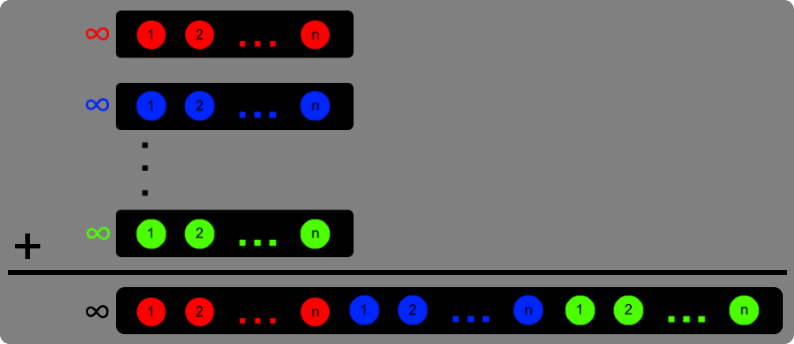
\includegraphics[scale=0.5]{Images/6.2.2.png}
\end{figure}

\newpage

{ \color{red} Theorem 6.2.3: The set of countable n-tuples are countable } 

	\begin{adjustbox}{minipage=14cm, right, vspace=0.1cm 0cm}
		Let A be a countably infinite set and B$_n$ be the set of all
		n-tuples ($a_1$,...,$a_n$) where $a_k$ $\in$ A.
		Then $B_n$ is countably infinite.
	\end{adjustbox}

{ \color{magenta} \underline{Proof} } 
	
	The base case $B_1$ is countably infinite since $B_1$ = A.

	Suppose $B_{n-1}$ is countably infinite. Then for every x $\in$ B:

	\qquad x = (b,a) \qquad \qquad b $\in$ $B_{n-1}$ and a $\in$ A

	Since for every fixed b, (b,a) $\sim$ A and thus, countably infinite.

	Since B is a set of countably infinite sets, then $B_{n}$
	is countably infinite. \\

{ \color{blue} Definition 6.2.4: $\mathbb{Q}$ is countably infinite } 

	\begin{adjustbox}{minipage=14cm, right, vspace=0.1cm 0cm}
		The set of rational numbers, $\mathbb{Q}$, is countably infinite.
	\end{adjustbox}

{ \color{magenta} \underline{Proof} } 
	
	Since elements of $\mathbb{Q}$ are of form $\frac{a}{b}$ which is a
	2-tuple, then by the {\color{red} theorem 6.2.3}, $\mathbb{Q}$ is countably infinite.

{ \color{magenta} \underline{Alternative Proof} } 
	
	For every x $\in$ $\mathbb{Q}$, let x = $(-1)^i$ $\frac{p}{q}$ where p,q $\in$ $\mathbb{Z}_+$.

	Let f(x) = $2^i$ $3^p$ $5^q$. Then by the Fundamental theorem of arithmetic,
	f is a 1-1 mapping of x to E $\subset$ $\mathbb{Z}_+$.

	Thus, $\mathbb{Q}$ is at most countable, but since p,q $\in$ $\mathbb{Z}_+$,
	then $\mathbb{Q}$ cannot be finite and thus, is countably infinite. \\

{ \color{purple} Example 6.2.5: Sequences of 0 and 1 are uncountable } 

	\begin{adjustbox}{minipage=14cm, right, vspace=0.1cm 0cm}
		Let A be the set of all sequences whose elements are digits 0 and 1.
		Then A is uncountable.
	\end{adjustbox}

{ \color{magenta} \underline{Proof: Cantor's Diagonalization Proof} } 

	Let set E be a countably infinite subset of A which consist of sequences $s_1,s_2,...$.

	Then construct a sequence s as follows:

	\qquad If the n-th digit in $s_n$ is 1, then let the n-th digit of s be 0
	and vice versa.

	Thus. s differs from every $s_n$ $\in$ E so s $\not \in$ E.

	But, s $\in$ A so E is a proper subset of A.

	Thus, every countably infinite subset of A is a proper subset of A.

	If A is countably infinite, then A is a proper subset of A which
	is a contradiction.



	